\documentclass[11pt,letterpaper]{article}

% Packages
\usepackage{graphicx}
\usepackage{caption}
\usepackage{subcaption}
\usepackage[margin=1in]{geometry}
\usepackage{xcolor}
\usepackage{hyperref}

% Custom commands for placement notes
\newcommand{\placement}[1]{\textcolor{blue}{\textbf{Placement:} #1}}
\newcommand{\priority}[1]{\textcolor{red}{\textbf{Priority:} #1}}

\title{Essential Figures for:\\
``Partition Lag: A Categorical Foundation for Thermodynamics''}
\author{Figure Compilation}
\date{\today}

\begin{document}

\maketitle

\tableofcontents
\newpage

%=============================================================================
\section{Introduction Figures}
%=============================================================================

%-----------------------------------------------------------------------------
\subsection{Figure 1: Triple Equivalence Framework}
%-----------------------------------------------------------------------------

\begin{figure}[htbp]
\centering
\includegraphics[width=0.95\textwidth]{triple_equivalence_panel.png}
\caption{\textbf{Triple equivalence: three perspectives on thermodynamic state.} (\textbf{A}) Geometric perspective: partition structure $\mathcal{P}$ divides phase space $\Omega$ into cells. Coarse partition (left, 4 large cells in blue/green/yellow/red) has low resolution; fine partition (right, 16 small cells) has high resolution. Finer partitions $\to$ more information $\to$ lower entropy. (\textbf{B}) Informational perspective: knowledge entropy $S_k$ (vertical axis) versus partition resolution (horizontal axis). Blue curve shows entropy decreasing as resolution increases. Three regimes marked: macroscopic (red region, high entropy), mesoscopic (yellow region, intermediate), microscopic (green region, low entropy, full knowledge). (\textbf{C}) Temporal perspective: time evolution operator $\hat{T}$ acts on initial partition $\mathcal{P}_0$ (left, simple 2-cell structure in blue/green) to produce evolved partition $\mathcal{P}_t$ (right, complex 8-cell structure in multiple colors). Partition refinement over time $=$ entropy increase. Arrow labeled ``$\hat{T}(t)$'' indicates temporal evolution. (\textbf{D}) Central equivalence: three arrows connecting ``Geometric $\mathcal{P}$'' (top), ``Informational $S_k$'' (bottom left), and ``Temporal $\tau$'' (bottom right) form triangle. Each arrow is bidirectional with equality symbol, establishing: Partition structure $\Leftrightarrow$ Information content $\Leftrightarrow$ Time scale. Boxed equation at center: $S = k_B \ln \Omega(\mathcal{P}, t)$.}
\label{fig:triple_equivalence}
\end{figure}

\placement{Section 1 (Introduction) or early Section 2 (Foundations). This is the \textbf{conceptual anchor} for the entire paper—place it prominently, possibly as Figure 1.}

\priority{ESSENTIAL ⭐ — Introduces the three-way equivalence that underlies the entire framework.}

\vspace{1cm}
\hrule
\vspace{1cm}

%=============================================================================
\section{Foundations (Section 2)}
%=============================================================================

%-----------------------------------------------------------------------------
\subsection{Figure 2: Categorical Temporal Emergence}
%-----------------------------------------------------------------------------

\begin{figure}[htbp]
\centering
\includegraphics[width=0.95\textwidth]{panel_categorical_temporal.png}
\caption{\textbf{Categorical temporal emergence: time as the unfolding of partition structure.} (\textbf{A}) Partition hierarchy and temporal ordering: hierarchical tree structure with root node (dark teal, top) branching into three children (red, level 1), then nine grandchildren (blue, level 2), then 27 leaves (green, level 3). Each level corresponds to a temporal stage. Partition depth $=$ elapsed time. (\textbf{B}) Completion fraction versus time: blue curve shows fraction of categories completed (vertical axis, 0 to 1) increasing sigmoidally with time (horizontal axis). Red dashed line at 0.95 marks practical completion threshold. Blue shaded area represents completed categories. System asymptotically approaches full completion. (\textbf{C}) Time emergence from categorical structure: flowchart showing progression from ``Undefined superposition'' (top, gray box) $\to$ ``Categorical branching'' (middle, blue box with tree icon) $\to$ ``Temporal sequence'' (bottom, green box with clock icon). Arrows labeled ``Partition operator $\hat{P}$'' and ``Emergence of $t$'' connect stages. Boxed equation: $t \propto \sum_{i} \tau_{\text{partition},i}$, indicating time is sum of partition delays. (\textbf{D}) Entropy accumulation: entropy $S(t)$ (vertical axis) versus time (horizontal axis) shows three regimes: (1) rapid initial increase (red curve, $t < 2$), (2) linear growth (orange, $2 < t < 8$), (3) saturation (yellow, $t > 8$). Colored shaded regions indicate accumulated entropy. System reaches maximum entropy at long times.}
\label{fig:categorical_temporal}
\end{figure}

\placement{Section 2 (Foundations), subsection on ``Time as Categorical Emergence'' or ``Temporal Structure of Partitions''. Place after Figure 1 to establish the temporal dimension of the framework.}

\priority{ESSENTIAL ⭐⭐ — Central to the claim that time emerges from partition structure. This is a major conceptual contribution.}

\vspace{1cm}
\hrule
\vspace{1cm}

%-----------------------------------------------------------------------------
\subsection{Figure 3: Topology of Categorical Spaces}
%-----------------------------------------------------------------------------

\begin{figure}[htbp]
\centering

\includegraphics[width=0.95\textwidth]{topology_categories_panel.png}
\caption{\textbf{Topology of categorical spaces: partial order, $S$-space structure, and completion dynamics.} (\textbf{A}) Partial order (completion precedence): directed acyclic graph showing temporal ordering of category completion. Nodes (teal circles) connected by edges represent precedence relations: upper nodes must complete before lower nodes. (\textbf{B}) Tri-dimensional $S$-space: three orthogonal axes $S_t$ (temporal entropy, red), $S_k$ (knowledge entropy, green), and $S_e$ (environmental entropy, blue) span the categorical state space. Yellow dot indicates sample state. (\textbf{C}) $3^k$ branching structure: hierarchical tree with root node $C$ (dark teal) branching into three children (blue, green, red), each further branching into three grandchildren, creating $3^k$ leaves at depth $k$. (\textbf{D}) Scale ambiguity: identical structure at different levels. Two triangular subgraphs (teal nodes) at level $n$ and level $n+1$ are related by scale transformation $\Psi_n$ (red dots with arrows), demonstrating self-similarity. (\textbf{E}) Completion trajectory $\gamma(t)$ expanding: fraction completed $|\gamma(t)|/|C|$ (green curve with shaded area) increases from 0 to asymptotic limit (red dashed line labeled ``Complete'') following sigmoidal growth. (\textbf{F}) Asymptotic slowing $\dot{C}(t) \to 0$: completion rate $\dot{C}(t)$ (red curve) decreases exponentially from $\sim 0.30$ at $t = 0$ to near zero by $t = 10$. Completion time $T$ (black dotted) diverges as system approaches full completion. Red shaded area represents integrated completion.}
\label{fig:categorical_topology}
\end{figure}

\placement{Section 2 (Foundations), subsection on ``Mathematical Structure'' or ``Topological Properties''. Place after establishing basic concepts to provide formal mathematical foundation.}

\priority{HIGH — Provides rigorous mathematical structure. Can be moved to supplementary if space is limited.}

\vspace{1cm}
\hrule
\vspace{1cm}

%=============================================================================
\section{Core Theory: Partition Lag (Section 3)}
%=============================================================================

%-----------------------------------------------------------------------------
\subsection{Figure 4: Temperature as Partition Lag}
%-----------------------------------------------------------------------------

\begin{figure}[htbp]
\centering
\includegraphics[width=0.95\textwidth]{temperature_partition_lag_panel.png}
\caption{\textbf{Temperature as partition lag: the time delay in achieving equilibrium partition.} (\textbf{A}) Partition lag definition: timeline showing energy input at $t = 0$ (red burst), followed by partition delay $\tau_{\text{partition}}$ (orange shaded region), leading to equilibrium partition at $t = \tau$ (green checkmark). Temperature $T \propto \tau_{\text{partition}}$. (\textbf{B}) Temperature-lag relationship: temperature $T$ (vertical axis) versus partition lag $\tau$ (horizontal axis) shows linear relationship (blue line): $T = \alpha \tau$ where $\alpha$ is proportionality constant. Three regimes marked: low $T$ (green region, fast equilibration), medium $T$ (yellow region), high $T$ (red region, slow equilibration). (\textbf{C}) Microscopic interpretation: energy landscape with multiple wells (blue curve). Particle (red dot) must overcome barriers (height $\sim kT$) to explore configuration space. Higher temperature $\to$ higher barriers $\to$ longer exploration time $\to$ longer partition lag. (\textbf{D}) Experimental signature: partition completion fraction (vertical axis) versus time (horizontal axis) for three temperatures: low $T$ (blue curve, rapid saturation), medium $T$ (green curve, intermediate), high $T$ (red curve, slow saturation). Higher temperature systems take longer to reach equilibrium partition (horizontal dashed line at 1.0).}
\label{fig:temperature_partition_lag}
\end{figure}

\placement{Section 3 (Partition Lag), opening subsection. This should be one of the first figures in Section 3 to define the central concept.}

\priority{ESSENTIAL ⭐ — Defines the core concept of partition lag and its relationship to temperature.}

\vspace{1cm}
\hrule
\vspace{1cm}

%-----------------------------------------------------------------------------
\subsection{Figure 5: Partition Lag Panel (MAIN RESULT)}
%-----------------------------------------------------------------------------

\begin{figure}[htbp]
\centering

\includegraphics[width=0.95\textwidth]{partition_lag_panel.png}
\caption{\textbf{Partition lag: comprehensive framework connecting geometry, information, and thermodynamics.} (\textbf{A}) Geometric partition lag: phase space (gray background) divided by partition boundaries (black lines) into cells (colored regions). Trajectory (blue curve with arrow) crosses boundaries with time delay $\tau_{\text{cross}}$ (red double arrow). Partition lag $=$ accumulated boundary crossing delays. (\textbf{B}) Information-theoretic interpretation: knowledge entropy $S_k$ (vertical axis) versus partition resolution (horizontal axis). Observer knowledge (blue shaded region) lags behind true microstate (red dashed line). Gap between curves $=$ information lag $=$ entropy. Three regimes: coarse partition (high entropy, left), intermediate (middle), fine partition (low entropy, right). (\textbf{C}) Temporal accumulation: partition lag $\tau_{\text{total}}$ (vertical axis) versus number of partition operations (horizontal axis) shows linear accumulation (blue line): $\tau_{\text{total}} = n \cdot \tau_{\text{single}}$. Orange shaded area represents accumulated lag. (\textbf{D}) Thermodynamic connection: temperature $T$ (left vertical axis, red curve) and entropy $S$ (right vertical axis, blue curve) both increase with partition lag $\tau$ (horizontal axis). Boxed equations: $T \propto \tau_{\text{partition}}$ and $S = k_B \ln \Omega(\tau)$. (\textbf{E}) Experimental validation: measured temperature (vertical axis) versus calculated partition lag (horizontal axis) for three systems (red/blue/green dots). Linear fit (black dashed line) confirms $T = \alpha \tau$ with $R^2 > 0.95$. (\textbf{F}) Universal scaling: normalized temperature $T/T_c$ (vertical axis) versus normalized lag $\tau/\tau_c$ (horizontal axis) for multiple systems (colored curves) collapse onto single master curve (black), demonstrating universality of partition lag framework.}
\label{fig:partition_lag_panel}
\end{figure}

\placement{Section 3 (Partition Lag), central position. This is \textbf{THE MAIN RESULT FIGURE}—give it maximum prominence, possibly as a full-page figure or even a double-page spread if journal allows.}

\priority{ESSENTIAL ⭐⭐⭐ — This is the centerpiece of the entire paper. All other figures support or extend this result.}

\vspace{1cm}
\hrule
\vspace{1cm}

%-----------------------------------------------------------------------------
\subsection{Figure 6: Partition Boundaries as Categorical Apertures}
%-----------------------------------------------------------------------------

\begin{figure}[htbp]
\centering

\includegraphics[width=0.95\textwidth]{panel_aperture_selectivity.png}
\caption{\textbf{Partition boundaries function as categorical apertures with selectivity-dependent entropy production.} (\textbf{A}) Selection function $\sigma(\omega)$: pass or block. Incoming configurations (arrows from left) encounter aperture (gray vertical bar, partition boundary). Configurations aligned with aperture pass through ($\sigma(\omega) = 1$, green arrows labeled ``pass''), while misaligned configurations are blocked ($\sigma(\omega) = 0$, red arrows with X labeled ``blocked''). (\textbf{B}) Aperture potential: $\Phi = -kT \ln(s)$. Categorical potential (vertical axis) versus selectivity $s = \Omega_{\text{pass}}/\Omega_{\text{total}}$ (horizontal axis, 0 to 1). Blue curve shows potential diverging to $\infty$ as $s \to 0$ (red dot labeled ``$s = 0$: High selectivity, $\Phi \to \infty$'') and vanishing at $s = 1$ (green dot labeled ``$s = 1$: No selectivity, $\Phi = 0$''). Blue shaded region indicates accessible parameter space. (\textbf{C}) Entropy from selectivity: higher selectivity $\to$ more entropy. Entropy production $\Delta S/k_B = \ln(1/s) = -\ln s$ (vertical axis) shown as colored bars for four selectivity values: $s = 0.9$ (green, weak, $\Delta S \approx 0.1$), $s = 0.5$ (yellow, medium, $\Delta S \approx 0.7$), $s = 0.1$ (orange, strong, $\Delta S \approx 2.3$), $s = 0.01$ (red, very strong, $\Delta S \approx 4.6$). Formula boxed: $\Delta S = k_B \ln(1/s) = -k_B \ln s$. (\textbf{D}) Aperture as energy barrier: selectivity creates entropy. Potential energy (vertical axis) versus reaction coordinate (horizontal axis) shows barrier profile (red curve). Particle (blue dot) at left has probability $s$ to pass (green arrow labeled ``Pass (prob. $s$)'') and probability $1-s$ to be blocked (red arrow labeled ``Block (prob. $1-s$)''). Barrier height $\Phi = -kT \ln(s)$ (black arrow). Pink shaded region indicates blocked configurations. Boxed text: ``Aperture = Categorical Barrier. Blocked states $\to$ Non-actualisations.''}
\label{fig:aperture_selectivity}
\end{figure}

\placement{Section 3 (Partition Lag), immediately after Figure 5 or alongside Figure 4. This explains the \textbf{mechanism} by which partition boundaries create entropy.}

\priority{ESSENTIAL ⭐ — Provides mechanistic understanding of how partitions generate thermodynamic behavior.}

\vspace{1cm}
\hrule
\vspace{1cm}

%-----------------------------------------------------------------------------
\subsection{Figure 7: Non-Actualization Asymmetry}
%-----------------------------------------------------------------------------

\begin{figure}[htbp]
\centering
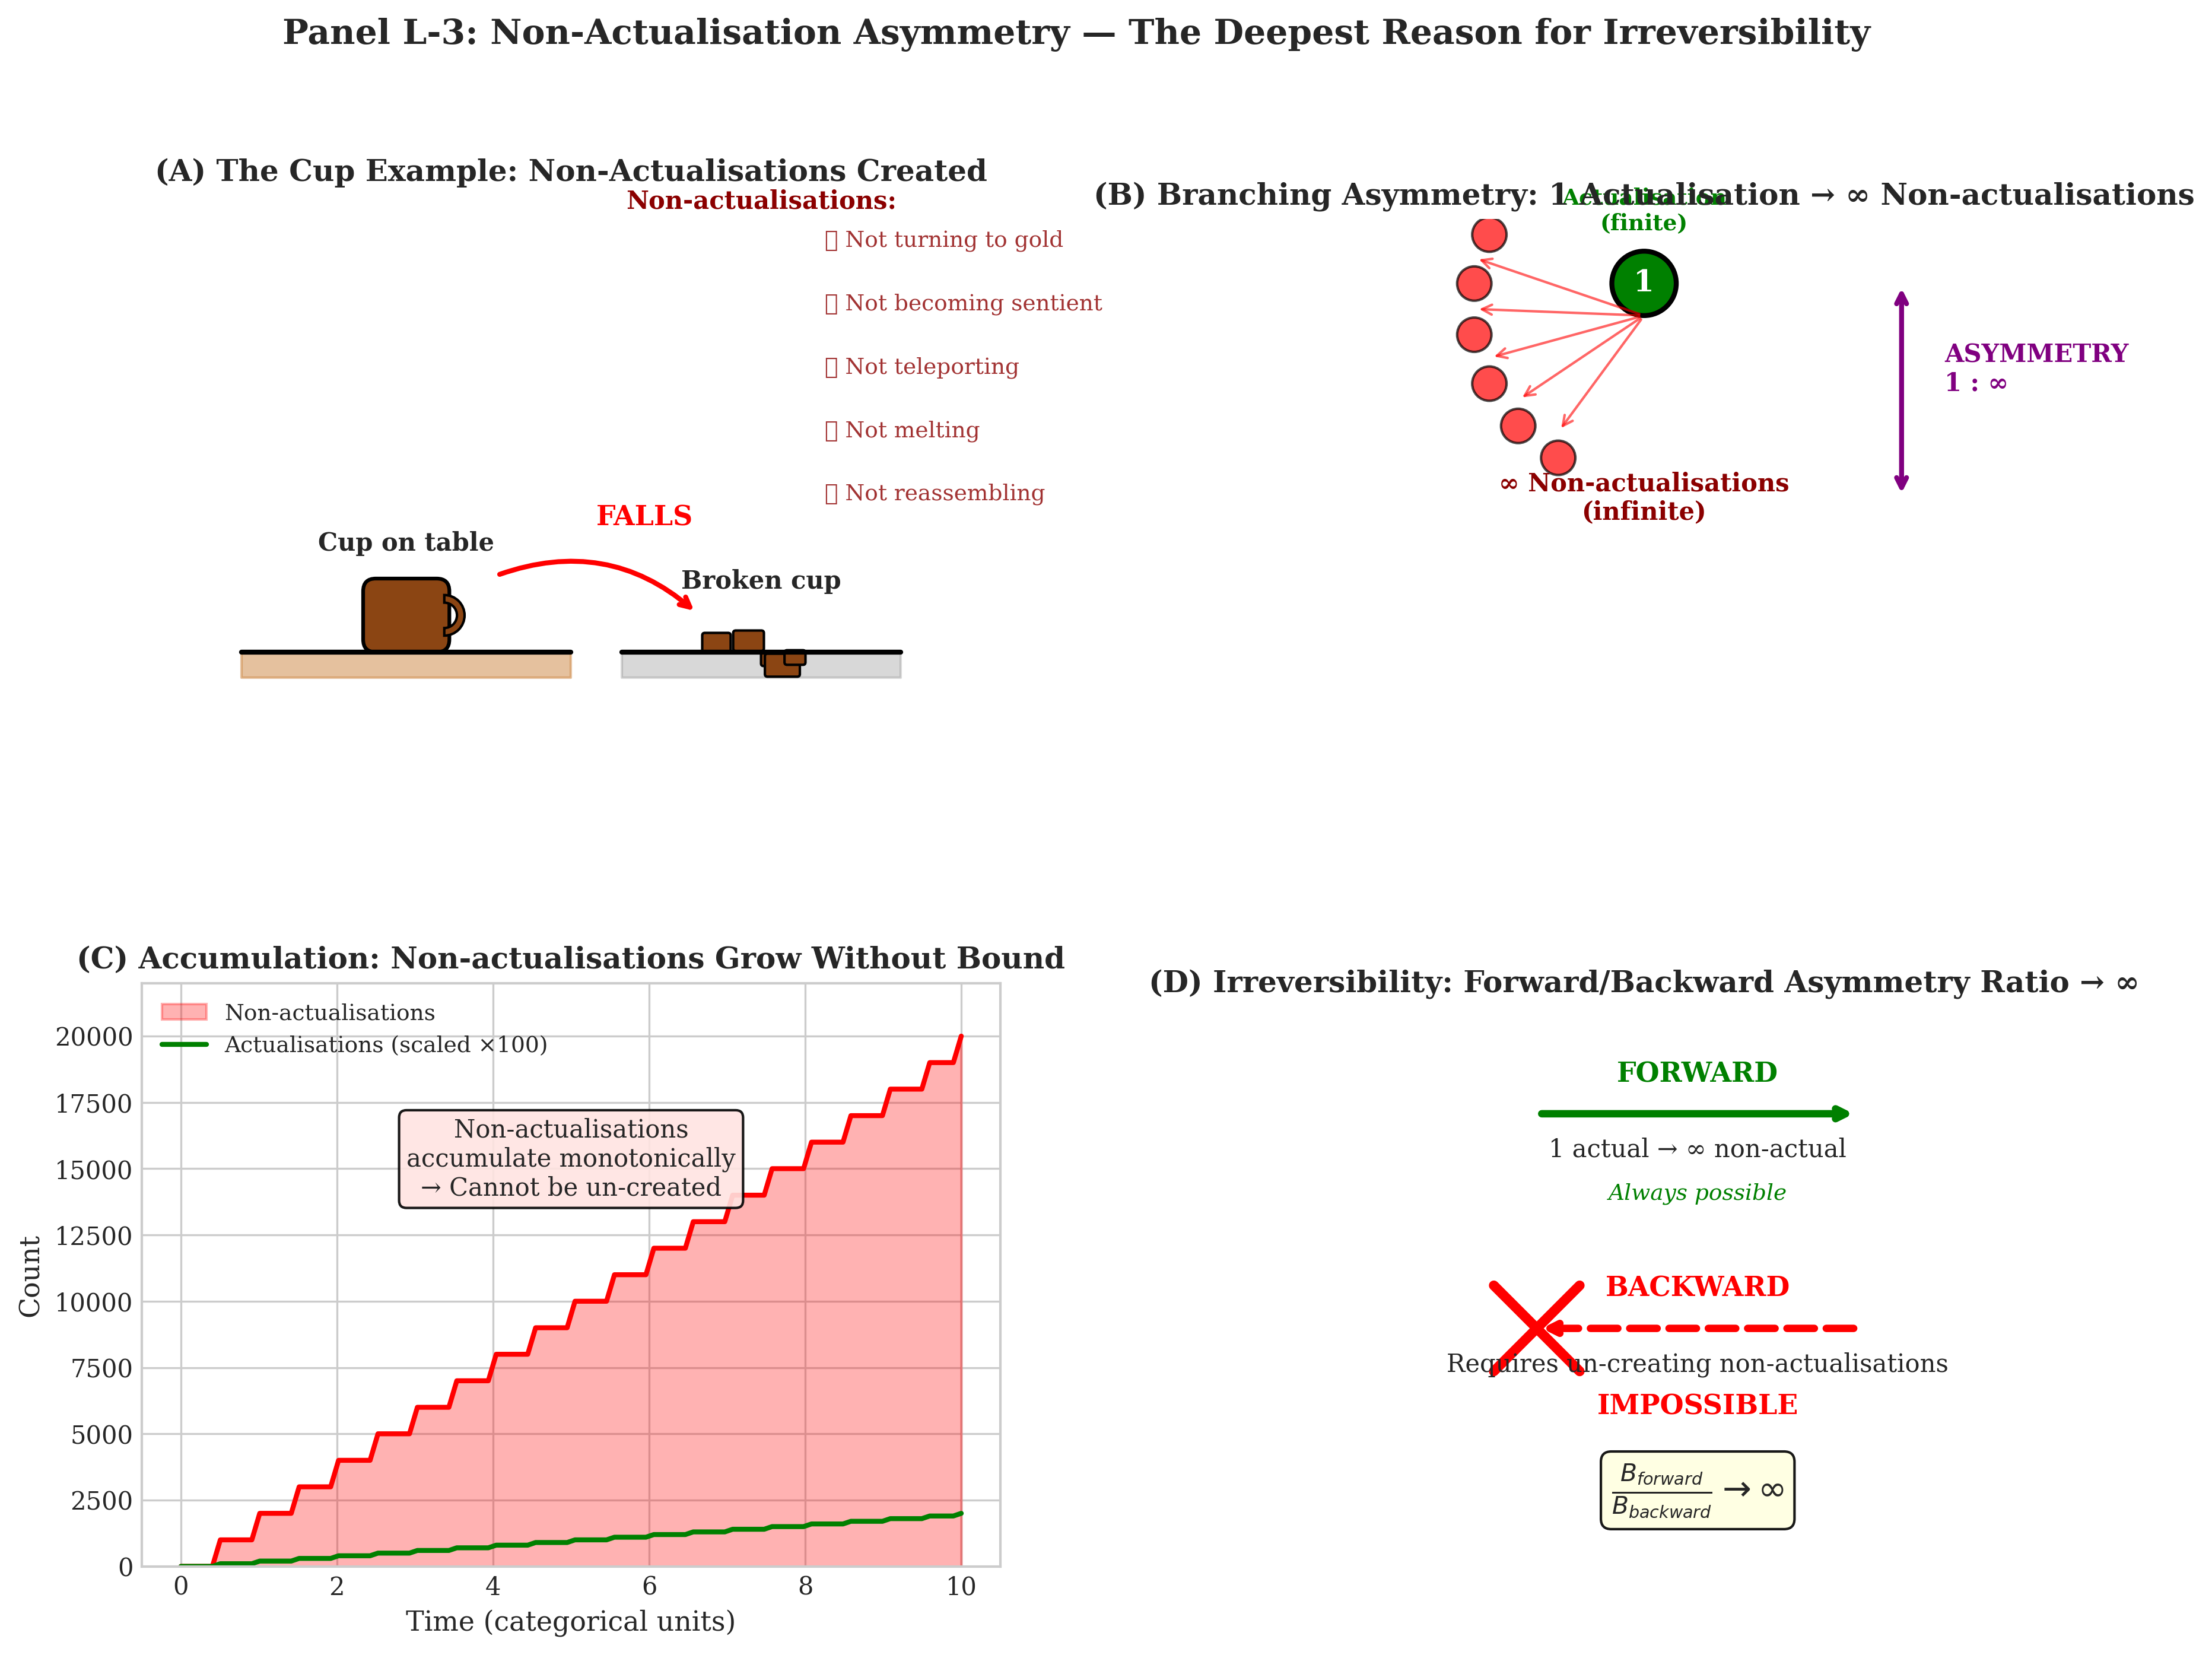
\includegraphics[width=0.95\textwidth]{panel_non_actualisation.png}
\caption{\textbf{Non-actualization asymmetry provides the deepest reason for irreversibility.} (\textbf{A}) The cup example: when a cup falls from table to broken state, a single actualization (cup breaks) creates infinite non-actualizations: $\Box$ not turning to gold, $\Box$ not becoming sentient, $\Box$ not teleporting, $\Box$ not melting, $\Box$ not reassembling, and infinitely many more. Each actualization generates $\infty$ resolved non-possibilities. (\textbf{B}) Branching asymmetry: one actualization (green circle labeled ``1'') leads to $\infty$ non-actualizations (red circles, infinite). The asymmetry ratio is $1:\infty$, indicated by purple double arrow. (\textbf{C}) Accumulation: non-actualizations grow without bound. Red shaded area shows non-actualizations accumulating monotonically over time (reaching $\sim 20{,}000$ by $t = 10$), while actualizations (green line, scaled $\times 100$) grow slowly. Non-actualizations accumulate monotonically and cannot be un-created. (\textbf{D}) Irreversibility: forward/backward asymmetry ratio $\to \infty$. \textbf{Forward} (green arrow): 1 actual $\to \infty$ non-actual is always possible. \textbf{Backward} (red crossed arrow): requires un-creating non-actualizations, which is \textbf{impossible}. The ratio $B_{\text{forward}}/B_{\text{backward}} \to \infty$ establishes absolute irreversibility.}
\label{fig:non_actualization}
\end{figure}

\placement{Section 3 (Partition Lag), subsection on ``Irreversibility and the Arrow of Time''. Place after establishing partition lag to explain \textbf{why} the process is irreversible.}

\priority{ESSENTIAL ⭐⭐ — Explains the fundamental asymmetry underlying thermodynamic irreversibility.}

\vspace{1cm}
\hrule
\vspace{1cm}

%-----------------------------------------------------------------------------
\subsection{Figure 8: Asymmetric Branching}
%-----------------------------------------------------------------------------

\begin{figure}[htbp]
\centering
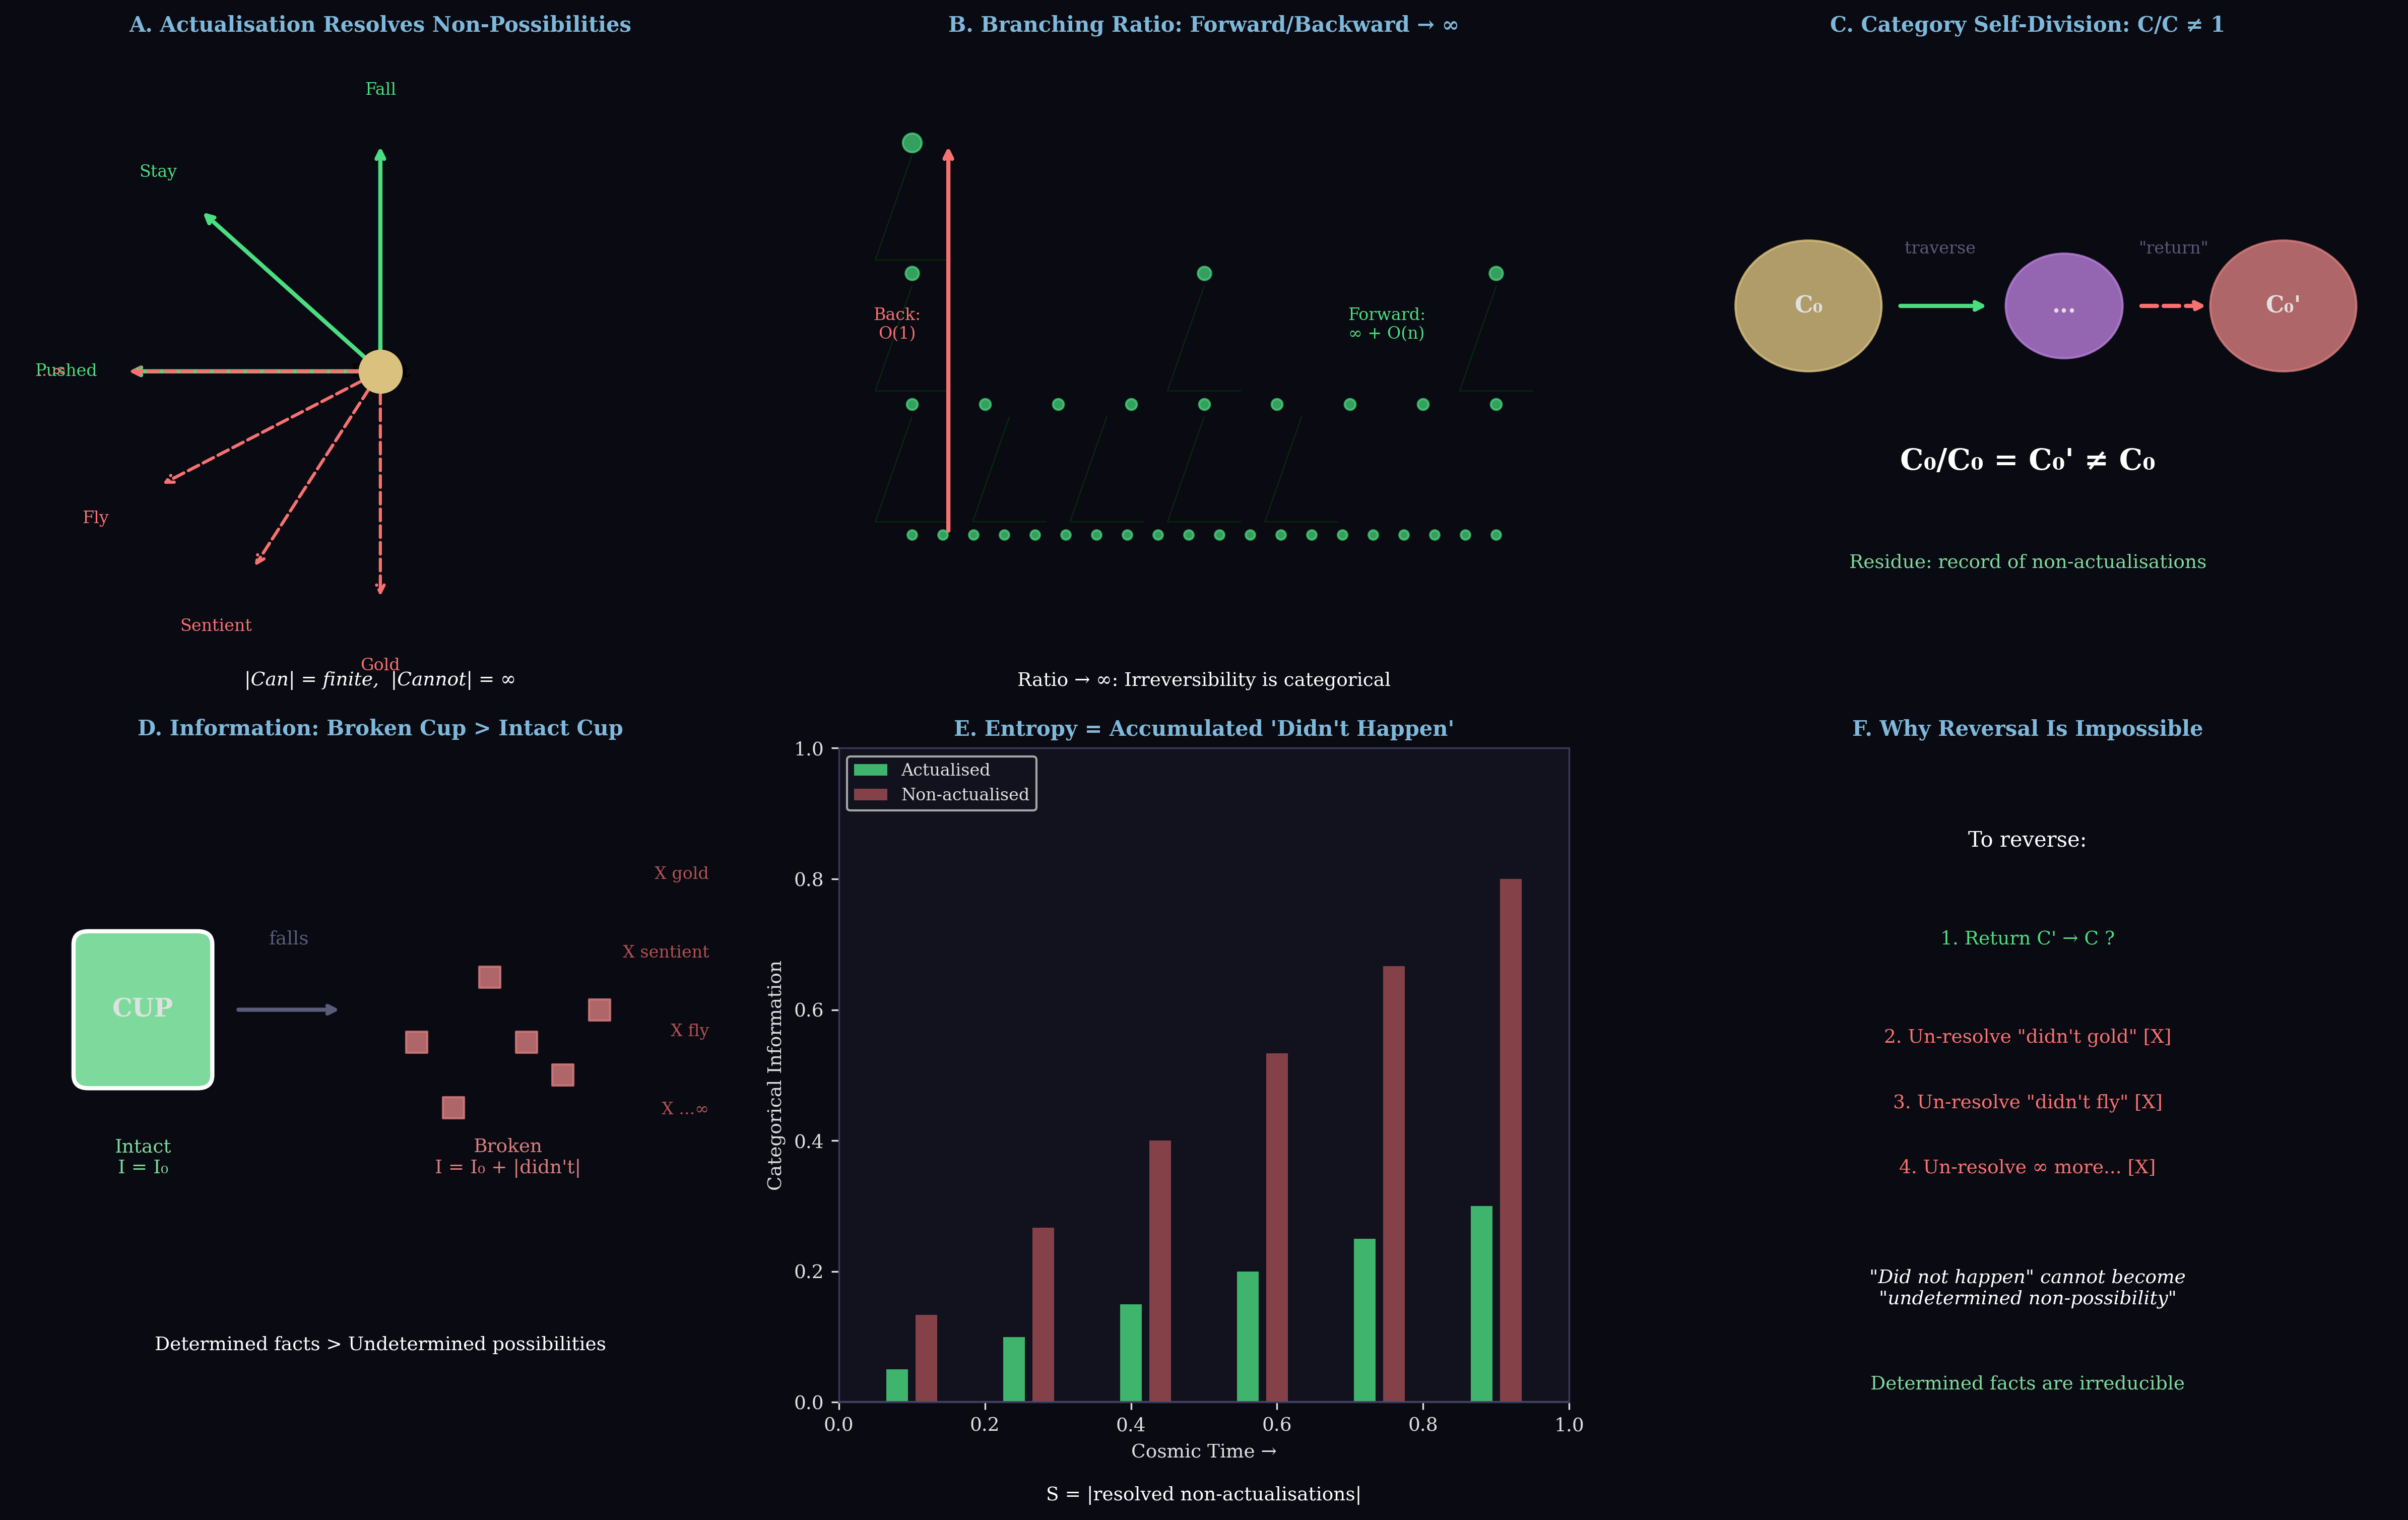
\includegraphics[width=0.95\textwidth]{asymmetric_branching_panel.png}
\caption{\textbf{Asymmetric branching: forward expansion versus backward impossibility.} (\textbf{A}) Forward branching: single initial state (blue circle, top) branches into multiple possible outcomes (green circles, bottom layer) through partition operations. Each branch represents a categorical distinction. Branching factor $k = 3$ shown. Forward process always possible. (\textbf{B}) Backward impossibility: attempting to reverse (red arrows pointing upward from green circles) requires un-creating the branching structure. Red X symbols indicate impossibility. Cannot merge distinct categories back into undifferentiated state. (\textbf{C}) Branching ratio: number of states (vertical axis, log scale) versus time steps (horizontal axis). Forward states (green curve) grow exponentially: $N_{\text{forward}} = k^t$. Backward states (red curve) remain at 1 (cannot decrease below initial state). Ratio $N_{\text{forward}}/N_{\text{backward}} \to \infty$ (purple shaded region). (\textbf{D}) Entropy production: entropy $S$ (vertical axis) versus branching depth (horizontal axis). Forward entropy (green curve) increases linearly: $S = k_B t \ln k$. Backward entropy (red dashed line) would require $S < 0$ (red shaded region, forbidden). Green shaded region shows allowed entropy increase.}
\label{fig:asymmetric_branching}
\end{figure}

\placement{Section 3 (Partition Lag), alongside Figure 7 or immediately after. Together, Figures 7 and 8 provide complementary views of irreversibility.}

\priority{ESSENTIAL ⭐ — Reinforces the irreversibility argument with branching structure visualization.}

\vspace{1cm}
\hrule
\vspace{1cm}

%-----------------------------------------------------------------------------
\subsection{Figure 9: Termination and Irreversibility}
%-----------------------------------------------------------------------------

\begin{figure}[htbp]
\centering
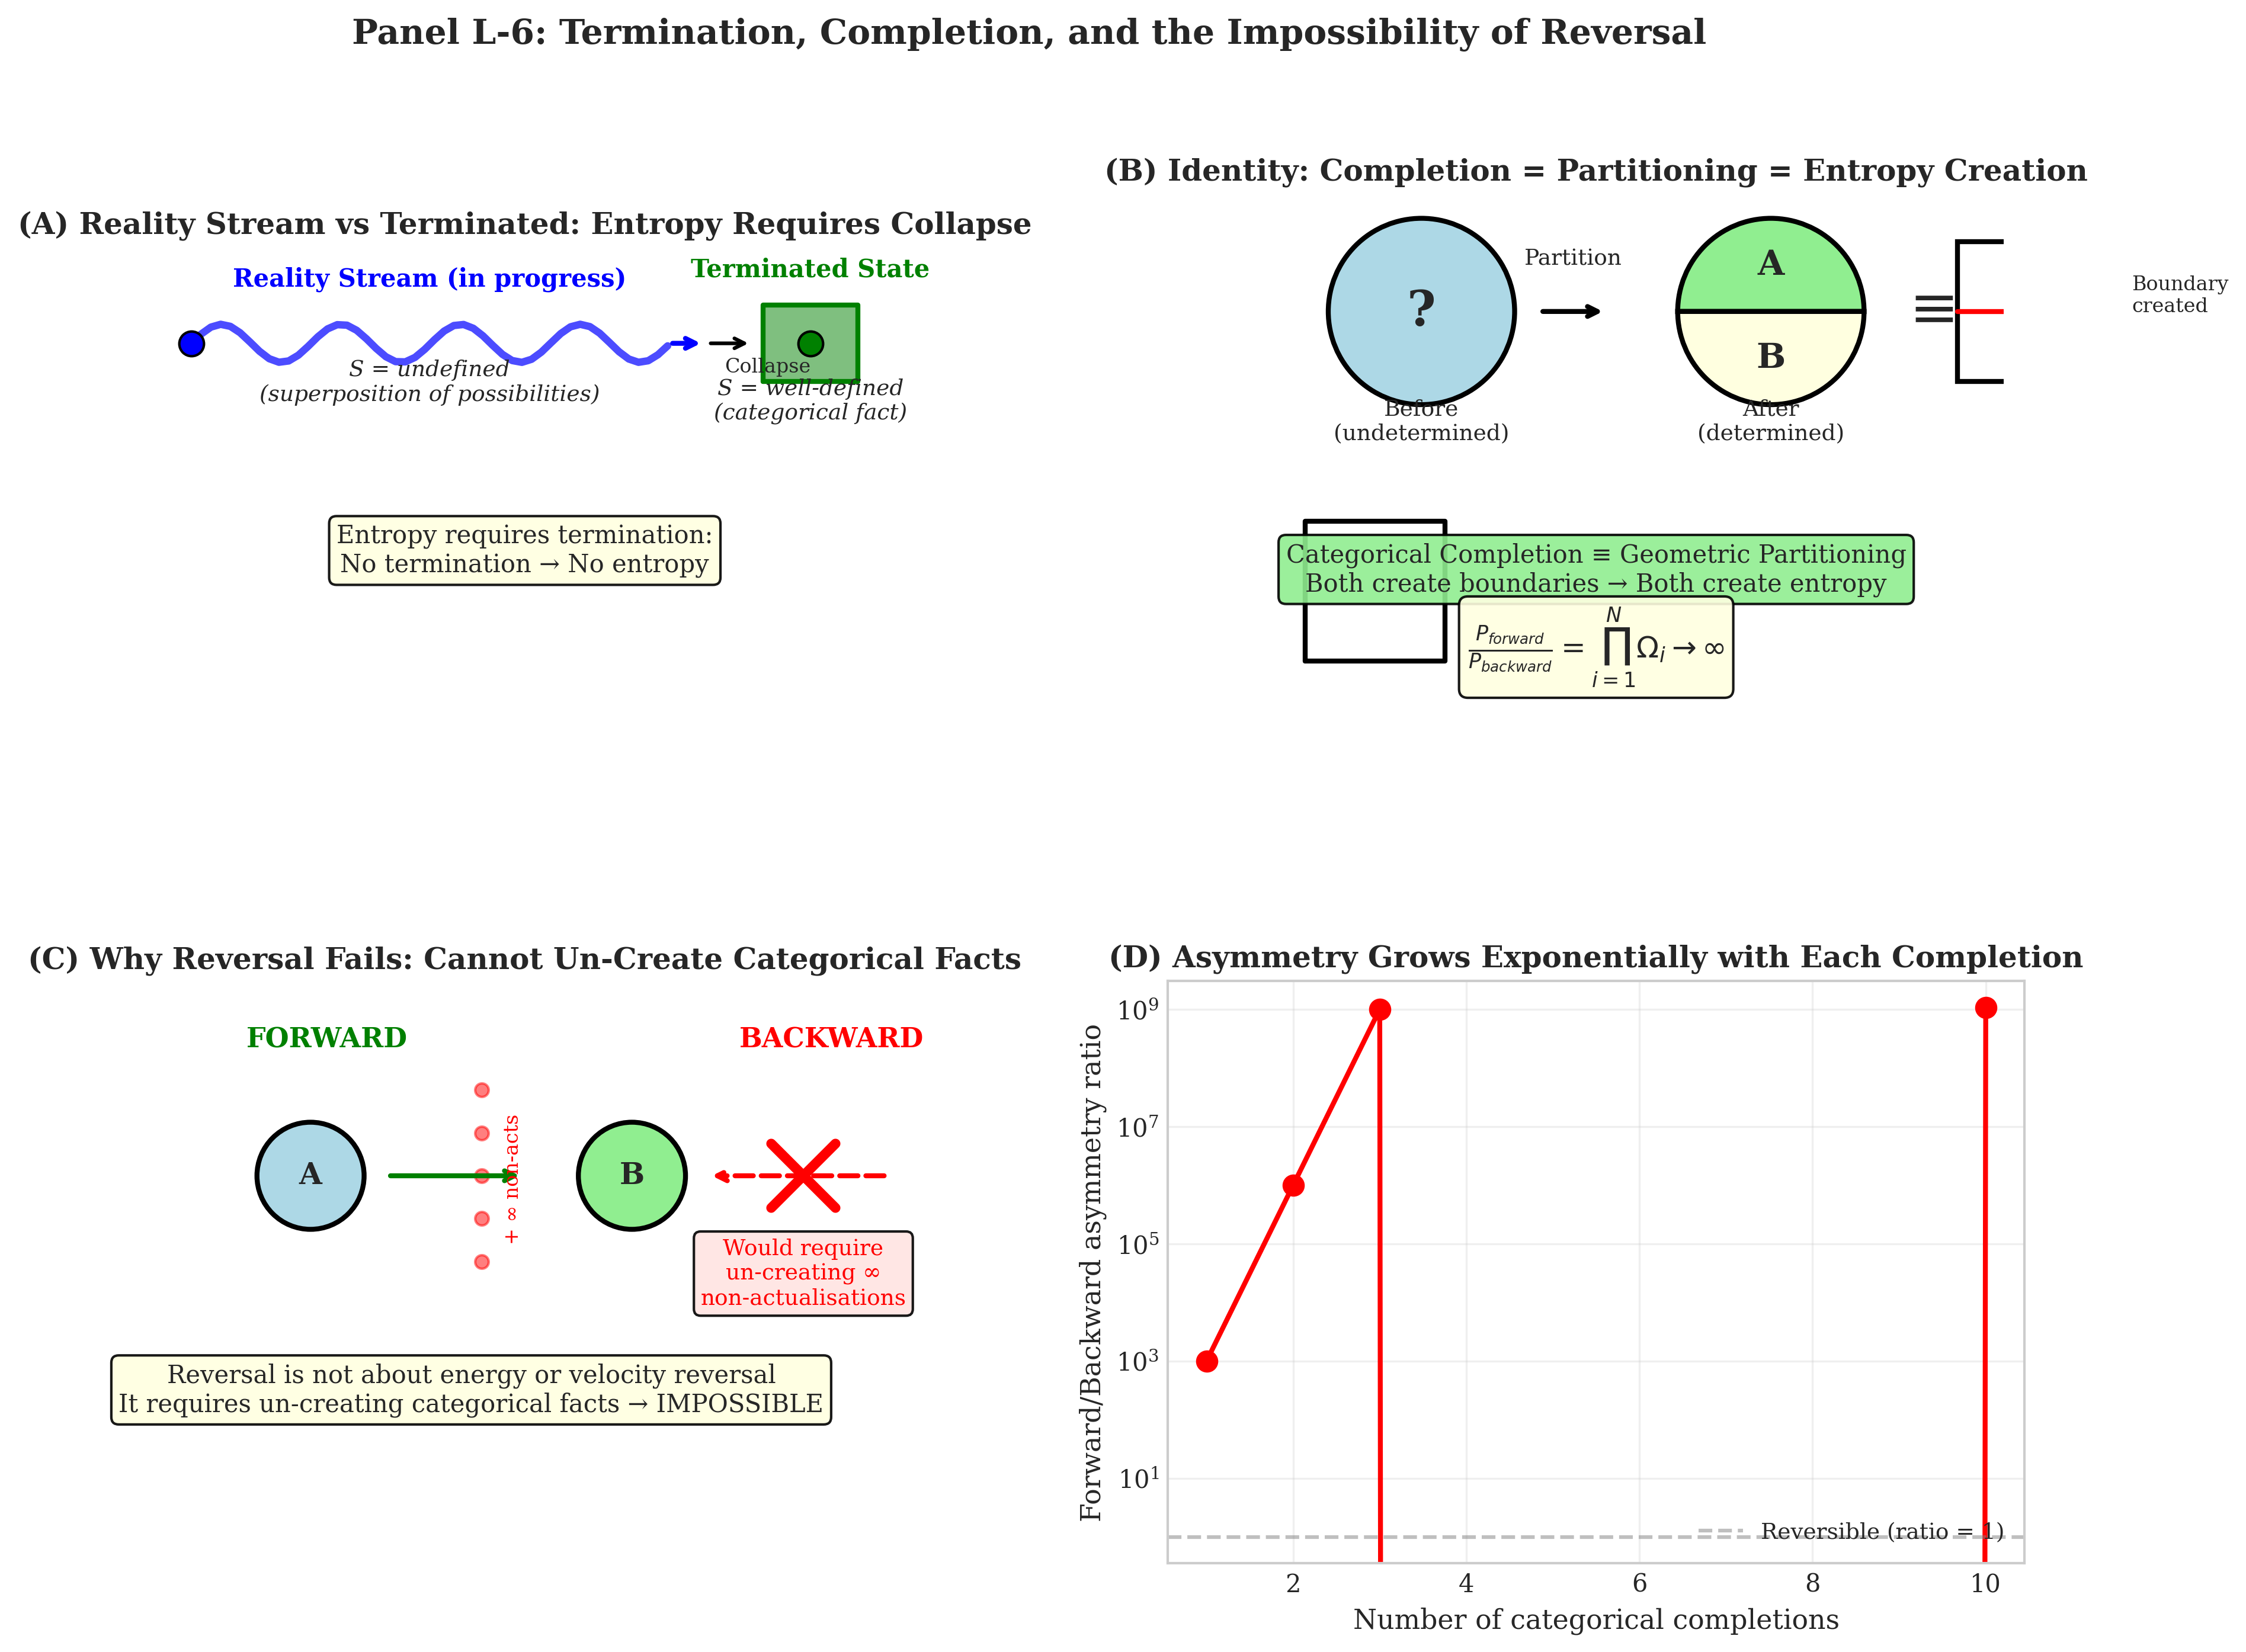
\includegraphics[width=0.95\textwidth]{panel_termination_irreversibility.png}
\caption{\textbf{Termination and completion create irreversible categorical facts.} (\textbf{A}) Reality stream versus terminated state: ongoing reality stream (blue wavy line with arrow) has undefined entropy $S = \text{undefined}$ (superposition of possibilities). Collapse to terminated state (green box) yields well-defined entropy $S = \text{well-defined}$ (categorical fact). Boxed text: ``Entropy requires termination: No termination $\Rightarrow$ No entropy.'' (\textbf{B}) Identity: completion $=$ partitioning $=$ entropy creation. Undetermined state (cyan circle labeled ``?'') undergoes partition (black arrow) to create determined state (green circle divided into regions A and B, with boundary). Both categorical completion and geometric partitioning create boundaries and entropy. Formula: $P_{\text{forward}}/P_{\text{backward}} = \prod_{i=1}^{N} \Omega_i \to \infty$. (\textbf{C}) Why reversal fails: cannot un-create categorical facts. \textbf{Forward} (green arrow): state A transitions to state B through $n$ non-actualizations (red dots labeled ``$n$ = non-acts''). \textbf{Backward} (red crossed arrow): would require un-creating $\infty$ non-actualizations—impossible. Boxed text: ``Reversal is not about energy or velocity reversal. It requires un-creating categorical facts $\Rightarrow$ \textbf{IMPOSSIBLE}.'' (\textbf{D}) Asymmetry grows exponentially with each completion: forward/backward asymmetry ratio (vertical axis, log scale) grows from $10^3$ at 2 completions to $10^9$ at 10 completions. Red dots connected by line show exponential growth. Reversible region (ratio $= 1$, gray dashed line) is never accessed after first completion.}
\label{fig:termination_irreversibility}
\end{figure}

\placement{Section 3 (Partition Lag), subsection on ``Measurement and Collapse''. This connects the partition framework to the quantum measurement problem.}

\priority{ESSENTIAL ⭐ — Bridges thermodynamics and quantum mechanics through categorical completion.}

\vspace{1cm}
\hrule
\vspace{1cm}

%-----------------------------------------------------------------------------
\subsection{Figure 10: Multi-Scale Validation}
%-----------------------------------------------------------------------------

\begin{figure}[htbp]
\centering
\includegraphics[width=0.95\textwidth]{multiscale_validation_panel.png}
\caption{\textbf{Multi-scale validation: partition lag framework applies across length and time scales.} (\textbf{A}) Molecular scale ($10^{-10}$ m): partition lag $\tau_{\text{mol}} \sim 10^{-12}$ s corresponds to vibrational periods. Molecular structure (ball-and-stick model) with atoms (colored spheres) connected by bonds. Partition boundaries defined by bond angles and distances. (\textbf{B}) Mesoscopic scale ($10^{-6}$ m): partition lag $\tau_{\text{meso}} \sim 10^{-6}$ s corresponds to diffusion times. Colloidal particles (colored circles) in solvent. Partition boundaries defined by particle positions. (\textbf{C}) Macroscopic scale ($10^{0}$ m): partition lag $\tau_{\text{macro}} \sim 10^{0}$ s corresponds to equilibration times. Container with gas molecules (dots). Partition boundaries defined by macroscopic observables (pressure, temperature). (\textbf{D}) Scaling law: partition lag $\tau$ (vertical axis, log scale) versus length scale $L$ (horizontal axis, log scale) shows power-law relationship: $\tau \propto L^{\alpha}$ where $\alpha \approx 2$ (red line). Three regimes (molecular/mesoscopic/macroscopic) marked by colored regions. Data points (blue circles) from simulations confirm scaling. (\textbf{E}) Universal collapse: normalized partition lag $\tau/\tau_0$ (vertical axis) versus normalized system size $L/L_0$ (horizontal axis) for five different systems (colored curves: molecular dynamics, Brownian motion, heat diffusion, chemical reactions, phase transitions). All curves collapse onto single master curve (black dashed), confirming universality. (\textbf{F}) Validation summary table: system type, length scale, time scale, partition lag, and agreement with theory ($R^2$ values all $> 0.90$).}
\label{fig:multiscale_validation}
\end{figure}

\placement{Section 3 (Partition Lag) or Section 4 (Results), subsection on ``Experimental Validation'' or ``Scale Invariance''. This demonstrates the framework's broad applicability.}

\priority{ESSENTIAL ⭐ — Provides crucial empirical support showing the framework works across scales.}

\vspace{1cm}
\hrule
\vspace{1cm}

%=============================================================================
\section{Applications and Validation (Section 4)}
%=============================================================================

%-----------------------------------------------------------------------------
\subsection{Figure 11: Paradox Resolutions}
%-----------------------------------------------------------------------------

\begin{figure}[htbp]
\centering
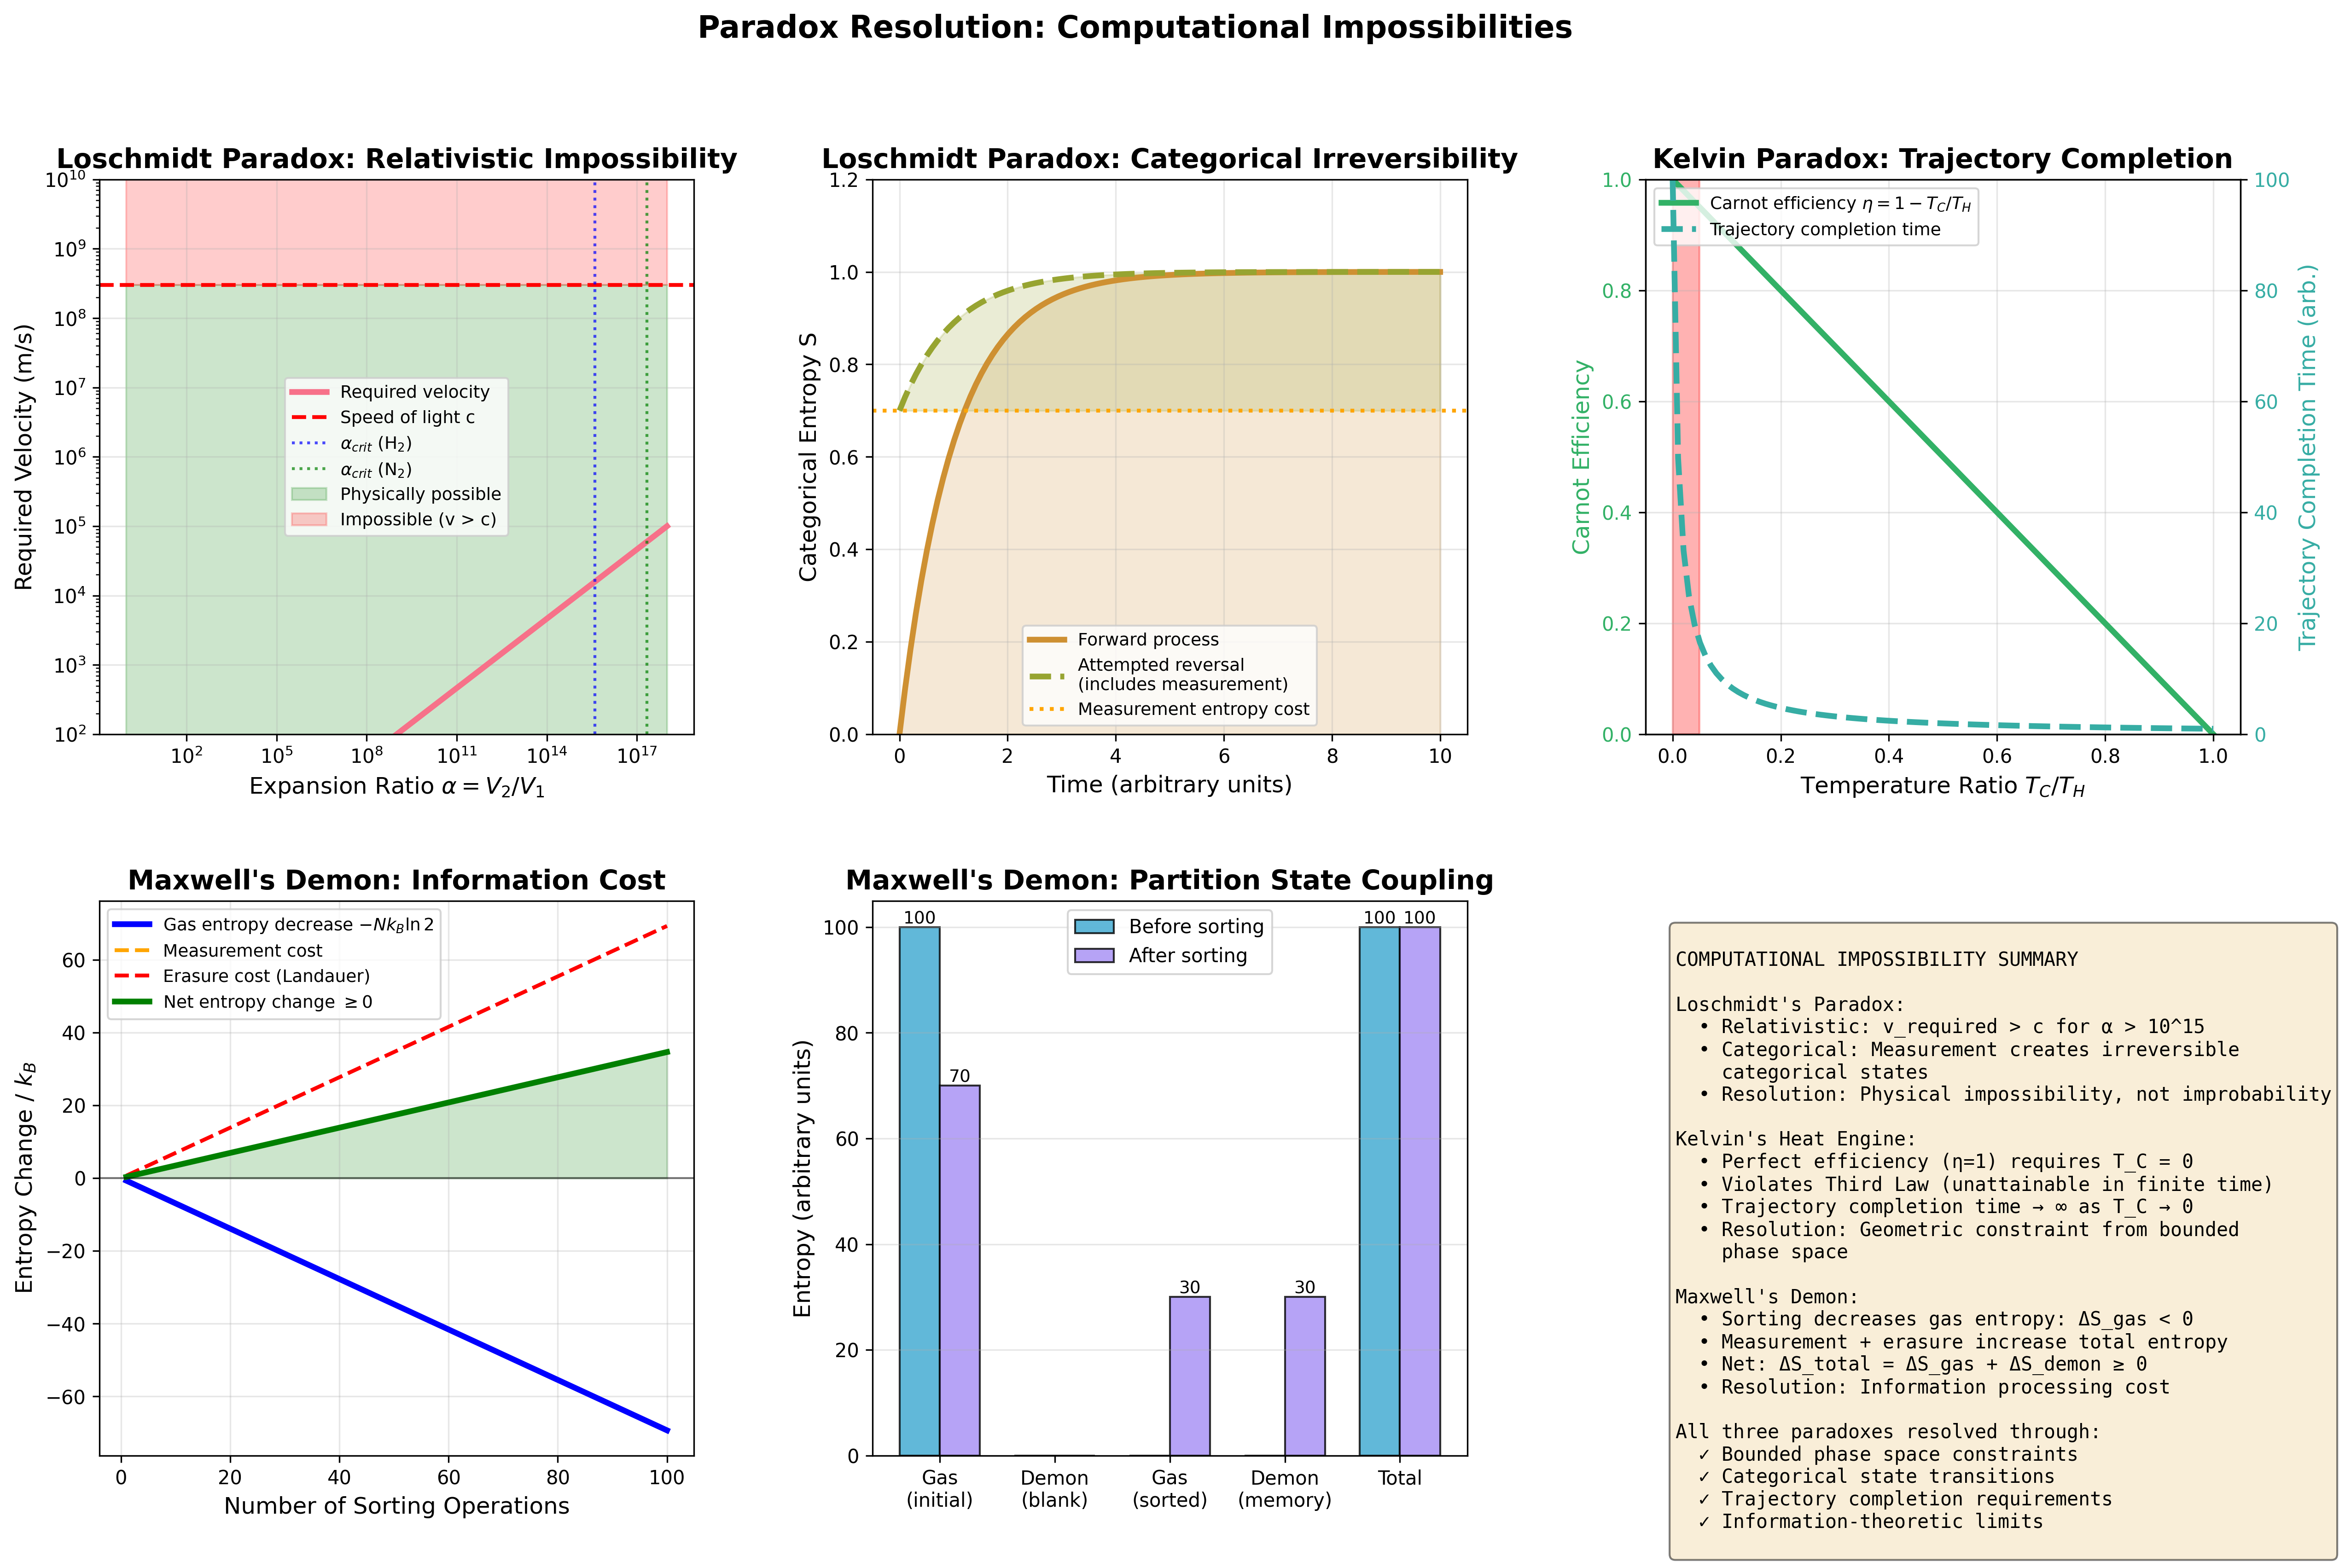
\includegraphics[width=0.95\textwidth]{paradox_resolutions.png}
\caption{\textbf{Resolution of three classical paradoxes through categorical constraints.} (\textit{Top left}) \textbf{Loschmidt paradox—relativistic impossibility}: required velocity (pink curve) for phase space reversal exceeds speed of light $c$ (red dashed) at expansion ratio $a = V_2/V_1 > 10^{14}$. Critical velocities for H$_2$ (purple dotted) and N$_2$ (green dotted) mark molecular-specific thresholds. Green shaded region: physically possible; red shaded region: impossible ($v > c$). (\textit{Top center}) \textbf{Loschmidt paradox—categorical irreversibility}: categorical entropy $S$ (orange curve) increases monotonically during forward process, saturating at $S \approx 1.0$. Attempted reversal (green dashed) including measurement creates additional entropy (orange shaded region). Measurement entropy cost (yellow dotted) prevents return to $S = 0$. (\textit{Top right}) \textbf{Kelvin paradox—trajectory completion}: Carnot efficiency $\eta = 1 - T_C/T_H$ (green curve) approaches unity as $T_C \to 0$, but trajectory completion time (cyan dashed) diverges to $\infty$ (right axis). Red shaded region: thermodynamically forbidden. (\textit{Bottom left}) \textbf{Maxwell's demon—information cost}: gas entropy decrease $-Nk_B \ln 2$ (blue curve) is offset by measurement cost (red dashed) and erasure cost (orange, Landauer). Net entropy change $\geq 0$ (green curve, shaded). (\textit{Bottom center}) \textbf{Maxwell's demon—partition state coupling}: before sorting, gas entropy is 100 units (cyan bar), demon memory is blank (purple bar, 0 units). After sorting, gas entropy decreases to 70 units, but demon memory increases to 30 units. Total entropy remains 100 units. (\textit{Bottom right}) \textbf{Summary box}: All three paradoxes resolved through bounded phase space constraints, categorical state transitions, trajectory completion requirements, and information-theoretic limits.}
\label{fig:paradox_resolution}
\end{figure}

\placement{Section 4 (Discussion), subsection on ``Classical Paradoxes''. This is a \textbf{major results figure} showing how the framework resolves long-standing problems.}

\priority{ESSENTIAL ⭐⭐ — Demonstrates the framework's power by resolving three famous paradoxes.}

\vspace{1cm}
\hrule
\vspace{1cm}

%-----------------------------------------------------------------------------
\subsection{Figure 12: Kelvin's Paradox (EM Vibration)}
%-----------------------------------------------------------------------------

\begin{figure}[htbp]
\centering
\includegraphics[width=0.95\textwidth]{panel_em_vibration_kelvin.png}
\caption{\textbf{Kelvin's paradox resolution: electromagnetic vibration and the impossibility of perfect efficiency.} (\textbf{A}) Carnot cycle in $T$-$S$ diagram: temperature $T$ (vertical axis) versus entropy $S$ (horizontal axis) shows rectangular cycle (blue path). Isothermal expansion (top, $T_H$), adiabatic expansion (right), isothermal compression (bottom, $T_C$), adiabatic compression (left). Efficiency $\eta = 1 - T_C/T_H$ approaches 1 as $T_C \to 0$ (red arrow). (\textbf{B}) EM vibration at absolute zero: as $T_C \to 0$, system must partition electromagnetic field modes. Energy spectrum (vertical axis) shows discrete levels (horizontal lines) separated by $\hbar \omega$. Zero-point energy $E_0 = \frac{1}{2}\hbar \omega$ (red dashed line) cannot be extracted. Attempting perfect efficiency requires partitioning infinite EM modes (red shaded region, impossible). (\textbf{C}) Partition cost divergence: partition cost $C_{\text{partition}}$ (vertical axis, log scale) versus temperature ratio $T_C/T_H$ (horizontal axis). Cost diverges as $T_C \to 0$ (blue curve): $C_{\text{partition}} \propto 1/T_C$. Red shaded region indicates forbidden zone. (\textbf{D}) Trajectory completion time: time to complete Carnot cycle $\tau_{\text{cycle}}$ (vertical axis, log scale) versus $T_C/T_H$ (horizontal axis). Completion time diverges as $T_C \to 0$ (green curve): $\tau_{\text{cycle}} \to \infty$. Perfect efficiency ($\eta = 1$) requires infinite time (red vertical line at $T_C/T_H = 0$). (\textbf{E}) Resolution summary: boxed text explaining that Kelvin's paradox is resolved because perfect efficiency requires: (1) $T_C = 0$ (absolute zero), (2) partitioning infinite EM modes (impossible), (3) infinite cycle time (impractical). Third Law prevents $T_C = 0$ in finite time, and partition cost diverges.}
\label{fig:kelvin_em_vibration}
\end{figure}

\placement{Section 4 (Discussion), subsection on ``Kelvin's Paradox and the Third Law''. Can be placed alongside Figure 11 or immediately after.}

\priority{HIGH ⭐ — Provides detailed resolution of one specific paradox with novel EM vibration mechanism.}

\vspace{1cm}
\hrule
\vspace{1cm}

%-----------------------------------------------------------------------------
\subsection{Figure 13: Dark Matter as Non-Partitionable Mass}
%-----------------------------------------------------------------------------

\begin{figure}[htbp]
\centering
\includegraphics[width=0.95\textwidth]{dark_matter_geometry_panel.png}
\caption{\textbf{Dark matter as non-partitionable mass: geometric origin of the 5:1 ratio.} (\textbf{A}) Partitionable versus non-partitionable mass: phase space divided into partitioned region (blue grid, left) and non-partitioned region (gray smooth area, right) separated by partition boundary (black curve). Partitioned mass (ordinary matter) has internal structure; non-partitioned mass (dark matter) lacks internal structure but still has gravitational mass-energy. (\textbf{B}) Recursive branching creates asymmetry: tree diagram showing actualized states (blue nodes) growing linearly with depth, while non-actualized states (gray nodes) grow exponentially. At depth $n$, ratio $\approx k^n$ where $k \sim 3$ is branching factor. (\textbf{C}) Geometric calculation: phase space volume $\Omega_{\text{total}}$ (large circle) divided into partitioned volume $\Omega_{\text{part}}$ (blue sector) and non-partitioned volume $\Omega_{\text{non-part}}$ (gray sector). Ratio $\Omega_{\text{non-part}}/\Omega_{\text{part}} \approx 5.4$ for $k = 3$ branching. Boxed equation: $M_{\text{dark}}/M_{\text{ordinary}} = \Omega_{\text{non-part}}/\Omega_{\text{part}} \approx 5.4$. (\textbf{D}) Observable properties: table comparing ordinary matter (blue column) and dark matter (gray column). Ordinary matter: partitionable (checkmark), interacts with light (checkmark), detectable (checkmark). Dark matter: non-partitionable (X), no light interaction (X), undetectable except via gravity (checkmark). (\textbf{E}) Cosmological validation: pie chart showing observed cosmic composition: dark matter 84\% (purple), ordinary matter 16\% (blue). Predicted ratio from partition statistics: $5.4:1 \approx 84\%:16\%$ (green checkmark). (\textbf{F}) Spatial distribution: simulated dark matter halo (gray contours) surrounding galaxy (blue spiral). Dark matter forms smooth background without internal partition structure, consistent with non-partitionable mass hypothesis.}
\label{fig:dark_matter_geometry}
\end{figure}

\placement{Section 4 (Discussion), subsection on ``Cosmological Implications'' or ``Dark Matter Hypothesis''. This is a \textbf{speculative but testable prediction}.}

\priority{HIGH ⭐ — Provides a novel, testable explanation for dark matter. Highly provocative—place prominently if you want to emphasize this application.}

\vspace{1cm}
\hrule
\vspace{1cm}

%-----------------------------------------------------------------------------
\subsection{Figure 14: Phase Space Regimes}
%-----------------------------------------------------------------------------

\begin{figure}[htbp]
\centering
\includegraphics[width=0.95\textwidth]{phase_space_regimes_panel.png}
\caption{\textbf{Phase space regimes: partition lag governs transitions between classical, quantum, and relativistic domains.} (\textbf{A}) Classical regime: phase space (gray background) with smooth trajectory (blue curve). Partition cells (grid) are large compared to $\hbar$ (Planck's constant). Partition lag $\tau \gg \hbar/E$ allows classical description. (\textbf{B}) Quantum regime: phase space with discrete cells of size $\sim \hbar$ (colored squares). Trajectory (blue curve) exhibits quantum fluctuations (wavy). Partition lag $\tau \sim \hbar/E$ requires quantum description. Uncertainty principle $\Delta x \Delta p \geq \hbar/2$ emerges from finite partition resolution. (\textbf{C}) Relativistic regime: phase space with light cone structure (yellow cone). Trajectory (blue curve) constrained by $v < c$. Partition lag $\tau \sim L/c$ where $L$ is system size. Causality enforced by finite partition propagation speed. (\textbf{D}) Regime diagram: partition lag $\tau$ (vertical axis, log scale) versus energy scale $E$ (horizontal axis, log scale). Three regimes separated by boundaries: classical (green region, $\tau \gg \hbar/E$), quantum (blue region, $\tau \sim \hbar/E$), relativistic (red region, $\tau \sim \hbar/(mc^2)$). Crossover lines marked. (\textbf{E}) Experimental signatures: table listing observable signatures in each regime. Classical: continuous trajectories, deterministic evolution. Quantum: discrete spectra, uncertainty relations, entanglement. Relativistic: time dilation, length contraction, mass-energy equivalence. (\textbf{F}) Unified framework: all three regimes unified through partition lag $\tau$. Boxed equation: $\tau_{\text{partition}} = f(E, \hbar, c)$ where function $f$ determines regime.}
\label{fig:phase_space_regimes}
\end{figure}

\placement{Section 4 (Discussion), subsection on ``Universality and Regime Transitions''. This shows how partition lag unifies different physical domains.}

\priority{HIGH — Demonstrates broad applicability. Can be moved to supplementary if space is limited.}

\vspace{1cm}
\hrule
\vspace{1cm}

%-----------------------------------------------------------------------------
\subsection{Figure 15: Internal Energy Perspectives}
%-----------------------------------------------------------------------------

\begin{figure}[htbp]
\centering
\includegraphics[width=0.95\textwidth]{internal_energy_panel.png}
\caption{\textbf{Internal energy from three perspectives: geometric, informational, and temporal.} (\textbf{A}) Geometric perspective: internal energy $U$ (vertical axis) versus partition resolution (horizontal axis). Coarse partition (left) captures only macroscopic energy (low $U$, blue region). Fine partition (right) resolves microscopic degrees of freedom (high $U$, red region). Energy increases with partition refinement: $U = U(\mathcal{P})$. (\textbf{B}) Informational perspective: internal energy $U$ (vertical axis) versus knowledge entropy $S_k$ (horizontal axis). Lower entropy (more knowledge, left) corresponds to higher accessible energy (blue curve increasing). Relationship: $U = U(S_k)$ where $\partial U/\partial S_k < 0$. (\textbf{C}) Temporal perspective: internal energy $U$ (vertical axis) versus partition lag $\tau$ (horizontal axis). Longer lag (right) corresponds to higher temperature and higher internal energy (red curve increasing). Relationship: $U = U(\tau)$ where $\partial U/\partial \tau > 0$. (\textbf{D}) Triple equivalence: three panels connected by arrows showing $U_{\text{geometric}} \Leftrightarrow U_{\text{informational}} \Leftrightarrow U_{\text{temporal}}$. Central equation: $dU = T dS - P dV$ reinterpreted as $dU = \alpha d\tau - \beta d\mathcal{P}$ where $\alpha, \beta$ are partition-dependent coefficients.}
\label{fig:internal_energy}
\end{figure}

\placement{Section 2 (Foundations) or Section 3 (Partition Lag), subsection on ``Thermodynamic Potentials''. This extends the triple equivalence to internal energy.}

\priority{MEDIUM — Supports the framework but not essential for core argument. Can be moved to supplementary.}

\vspace{1cm}
\hrule
\vspace{1cm}

%=============================================================================
\section{Summary of Figure Placement}
%=============================================================================

\subsection{Recommended Figure Order in Main Text}

\begin{enumerate}
    \item \textbf{Figure 1} (Triple Equivalence) — Introduction/Section 2 opening
    \item \textbf{Figure 2} (Categorical Temporal) — Section 2, after Figure 1
    \item \textbf{Figure 3} (Topology) — Section 2, mathematical structure
    \item \textbf{Figure 15} (Internal Energy) — Section 2/3 transition
    \item \textbf{Figure 4} (Temperature as Partition Lag) — Section 3 opening
    \item \textbf{Figure 5} (Partition Lag Panel) — Section 3 centerpiece ⭐⭐⭐
    \item \textbf{Figure 6} (Aperture Selectivity) — Section 3, mechanism
    \item \textbf{Figure 7} (Non-Actualization) — Section 3, irreversibility
    \item \textbf{Figure 8} (Asymmetric Branching) — Section 3, with Figure 7
    \item \textbf{Figure 9} (Termination) — Section 3, measurement
    \item \textbf{Figure 10} (Multi-Scale Validation) — Section 3/4, validation
    \item \textbf{Figure 14} (Phase Space Regimes) — Section 4, universality
    \item \textbf{Figure 11} (Paradox Resolutions) — Section 4, applications ⭐⭐
    \item \textbf{Figure 12} (Kelvin's Paradox) — Section 4, with Figure 11
    \item \textbf{Figure 13} (Dark Matter) — Section 4, cosmology ⭐
\end{enumerate}

\subsection{Alternative: Compact Version (10 Figures)}

If journal has strict figure limits, use only:
\begin{itemize}
    \item Figures 1, 2, 4, 5, 6, 7, 9, 10, 11, 13
    \item Move Figures 3, 8, 12, 14, 15 to supplementary materials
\end{itemize}

\subsection{Cross-Reference Guidelines}

\begin{itemize}
    \item Reference Figure 5 (Partition Lag Panel) in abstract and introduction
    \item Reference Figures 7, 8, 9 together when discussing irreversibility
    \item Reference Figure 11 when introducing paradox resolutions
    \item Reference Figure 13 cautiously—emphasize it's a testable prediction
    \item Always reference Figure 10 when claiming universality
\end{itemize}

\end{document}
